\chapter{Practical implementation}




During our research on stylization, we used Gratin which a pipeline rendering software using \textit{OpenGL}. It permits to easily creates rendered images with \textit{GLSL} combining previous images as textures <insert screenshot of gratin>. As we said before every texture used from our contribution can be computed in parallel on GPU including the noises, the fractalization of the noises, the alpha blending and the splatting. Our method use only images as input so it can easily be integrated into every pipeline rendering. For example, if you have a pipeline rendering with \textit{path tracing} to compute the color of your scene you can use this rendered image as color input of our method without re-compute it.\newline

\begin{figure}
    \begin{center}
    \fbox{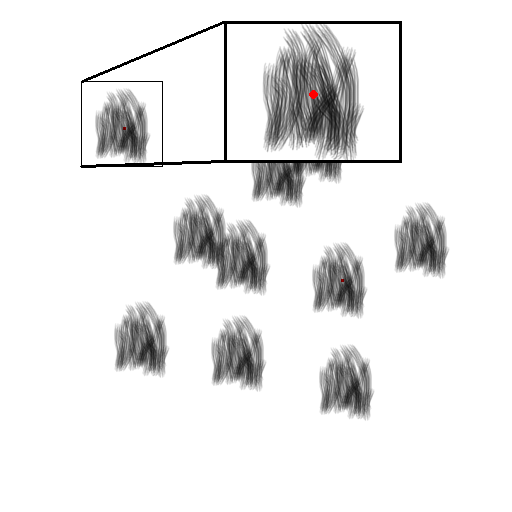
\includegraphics[width=60mm, height=60mm]{images/splatting/splatting4.png}}
    \end{center}
    \caption{Splatting principle: red dots are the anchor points.}
    \label{splatting_principle}
\end{figure}

For the splatting step, we draw on each pixel of the screen a square centered on the current pixel (see figure \ref{splatting_principle}). Every square is treated independently on the GPU before in the \textit{vertex shader} which manipulate the 4 vertices of the square which permits the resizing of the splat and permits the rotation of the splat. After this step of resizing and rotation, we pass in the \textit{fragment shader} which manipulate all pixels of splat. It is in this step that we will decide if we display the splat or not thanks to the procedural texture previously computed. \newline

\begin{figure}
    \begin{center}
    \fbox{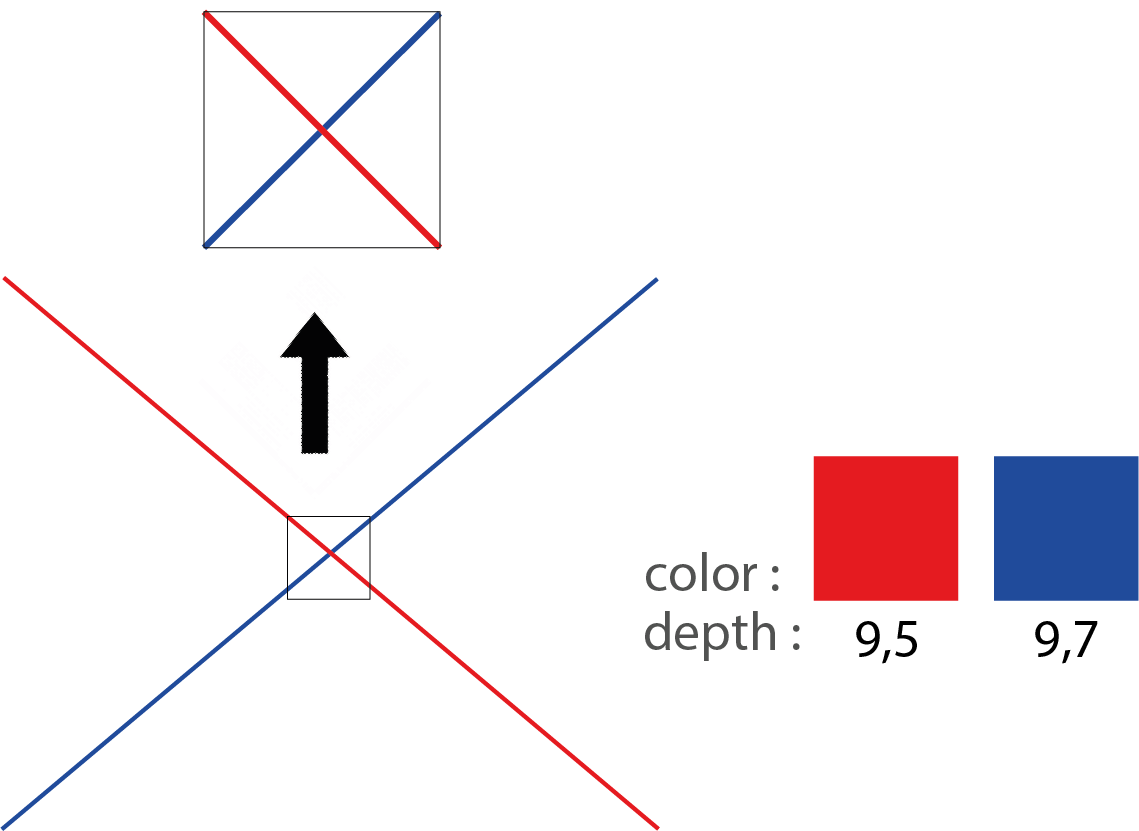
\includegraphics[scale=0.8]{images/splatting/order_independant_transparency.png}}
    \end{center}
    \caption{Example of usage of the order independant transparency.}
    \label{order}
\end{figure}

In this \textit{fragment shader}, we setup the technique of \textit{order-independent transparency} that consists to have in each pixel of the screen an array of color and depth (in our case the depth of the vertex where teh splat is anchored) in order to know which pixel is in front of the others pixels. In our example in the figure \ref{splatting_principle}, we have some splats that cover others splats. How do we know which one is in front the other if we treat them independently? For example, if there is a pixel where splat cover another one, we construct an array with 2 elements composed of a color and a depth so we can know which one is in front of the other one (see example in the figure \ref{order}).
